% The Editorial Office Requirements for the Table of Contents cause a significant problem 
%in Latex if there is only one Appendix. The Appendix is no longer labeled "A" in the TOC
%but has the word "APPENDIX" placed in front of the title of the Appendix. This can be done
%without issue IF nothing needs to be numbered by LaTeX in the Appendix. Unfortunately, most of the time
%something needs to be numbered in that single Appendix. For this reason we have included the IFTHENELSE switch
%found in this document and at the beginning of AppendixA. We assume that if you have any appendices, that you have more than one.
%So the default setting is noa = 2 (number of appendices = 2). Note: you don't need the actual number of appendices here
%1 or 2 are the only relevant numbers. You just make sure to input the Appendices you do have in this file.
%
%If, however, you DO only have one appendix change the line:
%
%\setcounter{noa}{2} to
%
%\setcounter{noa}{1}
%
%And comment (or delete) all of the input{AppendixB} commands except the first one.
%Then open the AppendixA.tex file and continue there.

%you can add/substract individual appendices through by using the /include{appendix'X'}
% and creating/deleting the appropriate files
\appendix %
\clearpage%
\newcounter{noa} % noa= no. of appendices ... set to 1 for 1 and more otherwise.
\setcounter{noa}{2} % ........................... CHANGE VALUE ONLY HERE
\ifthenelse{\value{noa} = 1}
%...................then
{}
%...................else
\addtocontents{toc}{\protect\addvspace{10pt}\noindent{APPENDIX}\protect\hfill\par}{}
%...................
%If you have a single appendix, you need to change {\chapter*{APPENDIX: THIS IS THE FIRST APPENDIX}
%to {\chapter*{APPENDIX: YOUR APPENDIX TITLE HERE} if you have two or more appendices
%you need to change {\chapter{THIS IS THE FIRST APPENDIX}} to
%{\chapter{YOUR APPENDIX TITLE HERE}}
%
%If you make these changes correctly Latex will complain bitterly about the additions to the TOC
%but will make them correctly in a manner acceptable to the Editorial Office.

\ifthenelse{\value{noa} = 1}
%...................then
{\chapter*{APPENDIX: STRUCTURED OVERLAY BROADCAST}
\label{broadcast}
\addcontentsline{toc}{chapter}{APPENDIX: STRUCTURED OVERLAY BROADCAST}
\chaptermark{Appendix}
\markboth{Appendix}{Appendix}
\setcounter{chapter}{1}}
%...................else
{\chapter{STRUCTURED OVERLAY BROADCAST}
\label{broadcast}}
%...................

\begin{figure}[ht]
\centering
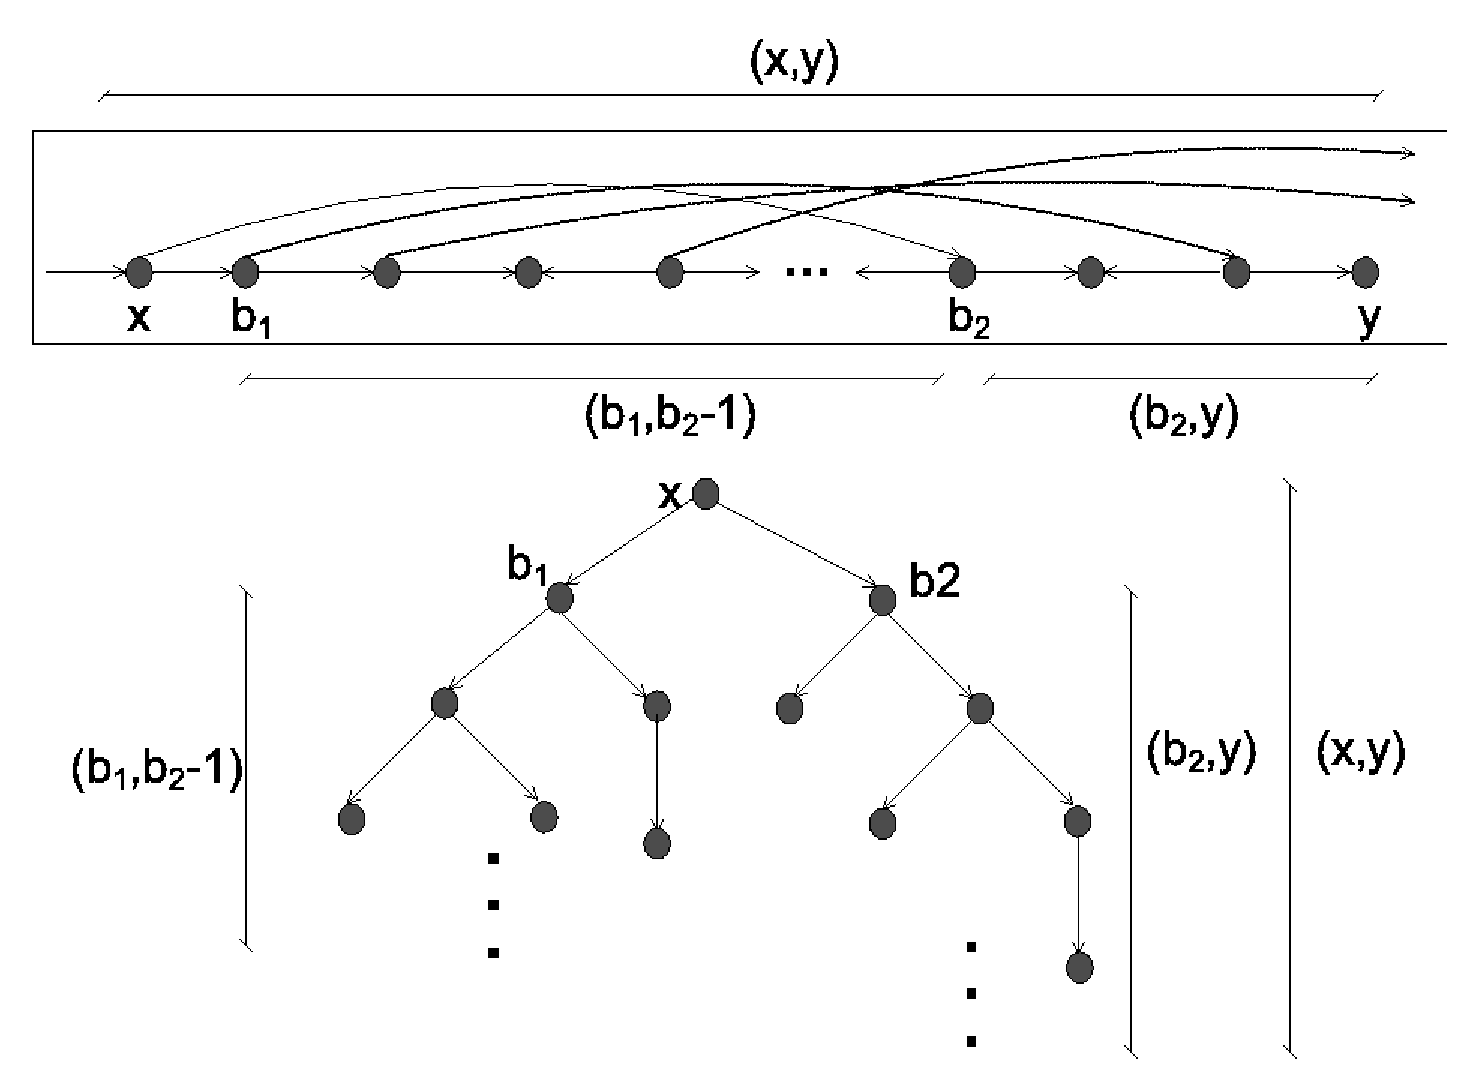
\includegraphics[width=4in]{figs/tree.eps}
\caption[Tree-based overlay broadcast]{Tree-based overlay broadcast}
\label{fig:tree}
\end{figure}  

Broadcast revocation can be used to address the deficiencies of DHT revocation.
As a topic of previous research works~\cite{broadcast, chord_broadcast},
structured overlays can be used without additional state to perform efficient
broadcasts from any point in the overlay to the entire overlay.  In these
papers, analysis and simulations have shown that the approach can be completed
in a network size of $n$ in $O(\log^2 n)$ time with $n$ messages.  The overlay
broadcast algorithm used in this paper provides a complete overlay broadcast in
$O(\log^2 n)$ time with $n$ messages.  When applied to Brunet, as illustrated
in Figure~\ref{fig:tree}, it utilizes the organization of a structured system
with a circular address space that requires peers be connected to those whose
node addresses are the closest to their own, features typical of
one-dimensional structured overlays including Chord~\cite{chord},
Pastry~\cite{pastry}, and Symphony.  Using such an organization, it is possible
to do perform a broadcast with no additional state.  To perform a broadcast,
each node performs the following recursive algorithm:

\begin{algorithmic}
\STATE {\bf BROADCAST(start, end, message)}:
  \STATE RECEIVE(message)
  \FOR{$i$ in length(connections)}
    \STATE n\_start $\gets$ ADDRESS(connections$[i]$)
    \IF {n\_start $\not\in$ $[$start, end$)$}
      \STATE continue
    \ENDIF
    \STATE n\_end $\gets$ ADDRESS(connections$[i+1]$)
    \IF {n\_end $\not\in$ $[$start, end$)$}
      \STATE n\_end $\gets$ end
    \ENDIF
    \STATE msg $\gets$ (BROADCAST, n\_start, n\_end, message)
    \STATE SEND(connections$[i]$, msg)
  \ENDFOR
\end{algorithmic}
with ``connections'' as a circular list of connections in non-decreasing order
from the perspective of the node performing the current recursive, broadcast
step.

In this algorithm, the broadcast initiator uses its own address as the start
and end, thus the broadcast will span the entire overlay after completing
recursive calls at each connected node.  A recursive end, ``n\_end'', must be
inside the region between ``start'' and ``end'', thus if the connection
following the current sending connection, ``connections$[i+1]$'', is not in
that region, it will only broadcast up to ``end'' and not the address specified
by that connection.  To summarize, the overlay is recursively partitioned
amongst the nodes at each hop in the broadcast.  By doing so, all nodes receive
the broadcast without receiving duplicate broadcast messages.

%If you have a single appendix, you need to change {\chapter*{APPENDIX: THIS IS THE FIRST APPENDIX}
%to {\chapter*{APPENDIX: YOUR APPENDIX TITLE HERE} if you have two or more appendices
%you need to change {\chapter{THIS IS THE FIRST APPENDIX}} to
%{\chapter{YOUR APPENDIX TITLE HERE}}
%
%If you make these changes correctly Latex will complain bitterly about the additions to the TOC
%but will make them correctly in a manner acceptable to the Editorial Office.

%\ifthenelse{\value{noa} = 1}
%...................then
%{\chapter*{APPENDIX: EVALUATION TOOLS}
%\label{evaluation_tools}
%\addcontentsline{toc}{chapter}{APPENDIX: EVALUATION TOOLS}
%\chaptermark{Appendix}
%\markboth{Appendix}{Appendix}
%\setcounter{chapter}{1}}
%...................else
{\chapter{EVALUATION TOOLS}
\label{evaluation_tools}}
%...................

Netperf~\cite{netperf} is used to estimate the latency and bandwidth of the
different VN models. The latency is measured by deploying Netperf in the
TCP\_RR mode, which measures the number of 1-byte request-receive transactions
that can be completed in a second. The bandwidth is estimated by running Netperf
in the TCP\_STREAM mode, which is a bulk transfer mode. It should be noted that
in situations where the link bandwidths were asymmetric, Netperf is deployed in
both directions.  Since both latency and bandwidth are dependent on the CPU
comparison, evaluations that include CPU utilization tasks require creating
a baseline first where only Netperf is the only active workload.

SPECjbb~\cite{specjbb} simulates a three-tier web application with all the
clients, the middle tier, and the database running on a single system in a
single address space (inside a JVM). On completion, the benchmark provides the
metric in terms of business of operations per second (bops). The bops score of
the system under test depends on both the CPU and the memory in the system, as
the entire database for the benchmark is held in memory. This benchmark
generates negligible disk activity and no network activity. 

